\documentclass[aps,pra,notitlepage,amsmath,amssymb,letterpaper,12pt]{revtex4-1}
\usepackage{amsthm}
\usepackage{graphicx}
%  Above uses the Americal Physical Society template for Physical Review A
%  as a reasonable and fully-featured default template
 
%  Below define helpful commands to set up problem environments easily
\newenvironment{problem}[2][Problem]{\begin{trivlist}
\item[\hskip \labelsep {\bfseries #1}\hskip \labelsep {\bfseries #2.}]}{\end{trivlist}}
\newenvironment{solution}{\begin{proof}[Solution]}{\end{proof}}
 
% --------------------------------------------------------------
%                   Document Begins Here
% --------------------------------------------------------------

% In what follows, you can easily change text to see what happens to the document
% For example, replacing the text "Document X" inside the "\title{}" command will
% change the document title
 
\begin{document}
 
\title{The Sombrero Function: Duffing Oscillators}
\author{Trevor Kling}
\affiliation{PHYS 220, Schmid College of Science and Technology, Chapman University}
\date{\today}

\maketitle

\section{Introduction}

For a ball moving with slight friction, the potential as a function of distance $x$ can be described by the function $V(x) = x^4/4 - x^2/2$.  This function is sometimes referred to as a "sombrero," due to its high central peak and distal troughs. In this module, a rolling ball described by this function is given a slight driving force $F$.  This causes the system to be able to be re-written as
$$m\ddot{x} = f_{\text{hat}}(x) + f_{\text{drag}}(\dot{x}) + f_{\text{drive}}(t) = x - x^3 - \nu \dot{x} + F\cos(\omega t)$$
which can subseqently be broken into a system of differential equations,
$$\dot{x}(t) = y(t)$$
$$m\dot{y}(t) = -\nu y(t) + x(t) - x^3(t) + F\cos(\omega t)$$
This system is then solved using the Fourth-Order Runge-Kutta method, and graphed as a parametric curve $(x(t), y(t))$.  The effect of various forces and starting positions on the Duffing Oscillator is then examined.

\section{Implementation}

The function was subsequently implemented in Python, to facilitate generation of values and graphing.  The program used a fixed range $t \in [0,2\pi N]$, with a step size of $0.001$ to generate a sufficiently accurate data set for a continuous function.  The values of $F$, $x_0$, and $y_0$ are varied to produce comparable results.  Each of these functions is graphed, and the structure of the graph is compared via a Poincare Section of the graph.

\section{Analysis}
\subsection{Graph 1: Linear}

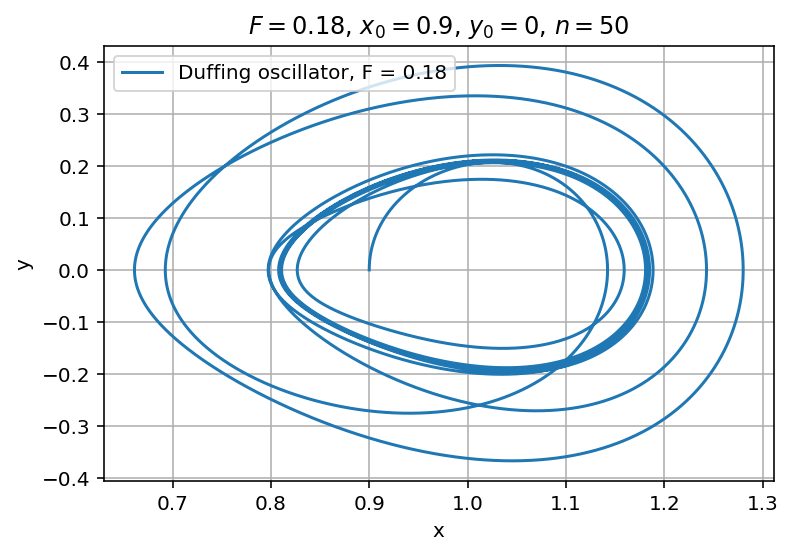
\includegraphics{graph1.png}

The first of the graphs features a driving force of $0.18$, and produces a smooth, egg-like shape.  It can clearly be seen that the function is periodic, with a slight deviation due to the driving force.

\subsection{Graph 1: Poincare}

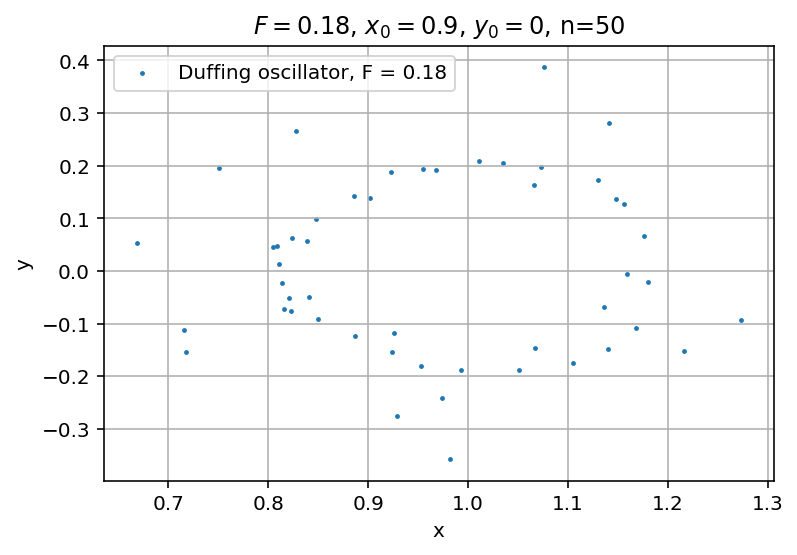
\includegraphics{poincare1.png}

To better analyze this graph, a Poincare section of the curve is also generated for all $t$ values where $t = 2\pi n \text{, } 0 \leq n \leq 50$. From this graph, it can be seen that a great deal of the points are concetrated in an elipse-like shape around the center point $(-1.00, 0)$ with far fewer points inside our outside the elipse.  This likely represents the ball falling into one of the "troughs" of potential, and only being shaken back and forth a bit when the driving force increases.

\subsection{Graph 2: Linear}

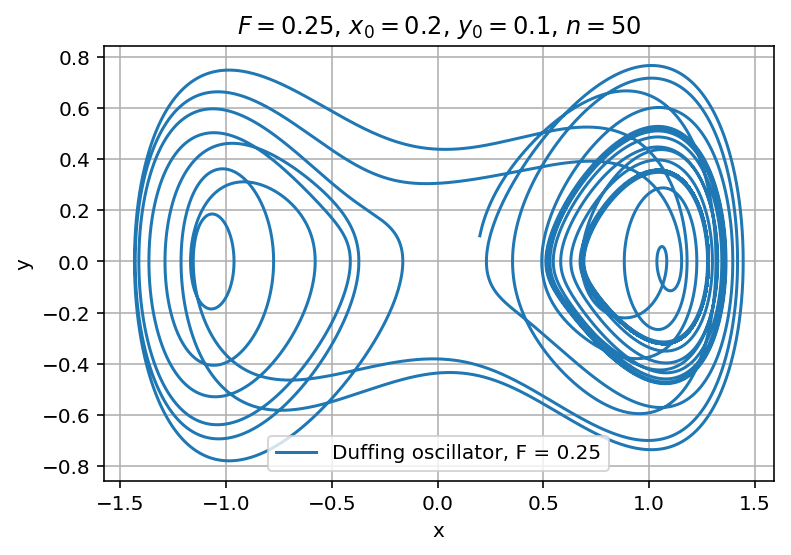
\includegraphics{graph2.png}

For the next graph, the same system is analyzed with a positive $x_0$ value.  Interestingly, the loop moves the opposite direction and is substantially more prone to diverging from the most solid loop.  The change of direction is likely caused by the ball being moved to the opposite side of the sombrero, causing it to roll down into the other trough.

\subsection{Graph 2: Poincare}

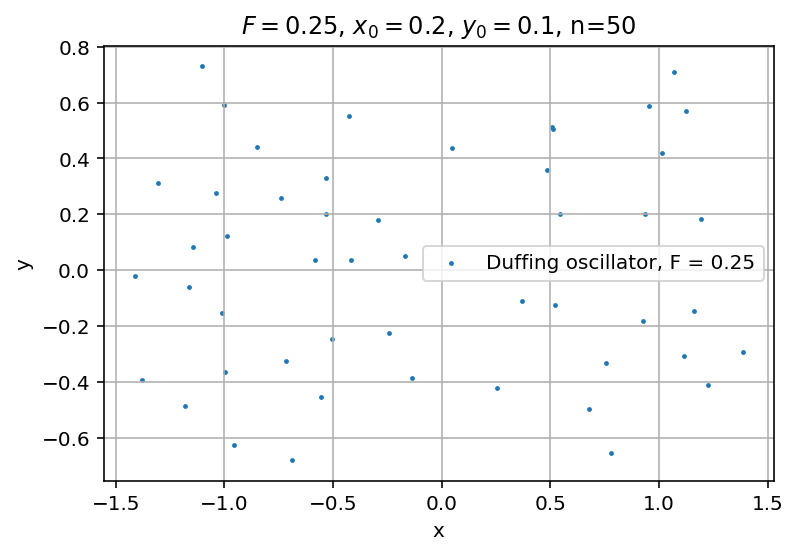
\includegraphics{poincare2.png}

The Poincare section shows a similar result to before, but with a less convergent result.  Points seem to scatter farther due to the driving force when the $x_0$ is positive than when it is negative.  This is likely due to the fact that the driving force is always positive, and the slope of the outer edge of the trough is not a steep as the slope of the peak of the sombrero.  Therefore, attempting to push the ball up the more gradual slope with the same force will result in a larger distance traveled.

\subsection{Graph 3: Linear}

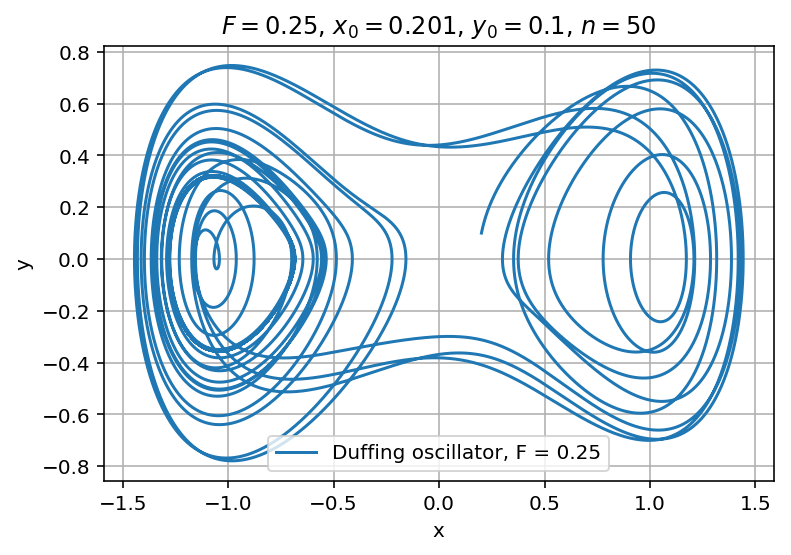
\includegraphics{graph3.png}

For the final graph, the same system is analyzed with a positive $x_0$ value.  Interestingly, the loop moves the opposite direction and is substantially more prone to diverging from the most solid loop.  The change of direction is likely caused by the ball being moved to the opposite side of the sombrero, causing it to roll down into the other trough.

\end{document}
